\documentclass[11pt]{article}
\usepackage{graphicx}
\usepackage{listings}
\usepackage[margin=1in]{geometry}
\usepackage{placeins}
\usepackage{float}

\author{Andrew Smith, Kofi Otseidu, Manav Trivedi}
\title{Machine Learning}

\begin{document}
\maketitle

\section{Predicting which officers will recieve complaints}

\section{Predicting the cost of a settlement}
So for this problem, we first create a feature matrix. Included as features are the officer rank, age (at time of settlement), gender, race, awards, neighborhood, and number of complaints and settlements prior to the current settlement. From that we use a regression to try to predict the cost of a settlement. We used a generalized linear model with a log-gaussian fit. We used cross validation to refine the hyperparameters and output the best model.

Looking at the result on test data, the predicted data distribution generally matches the actual distribution. Below are some of the plots, and the code will be up on our github.

\begin{figure}[h]
\centering
\caption{Predicted Settlement Values}
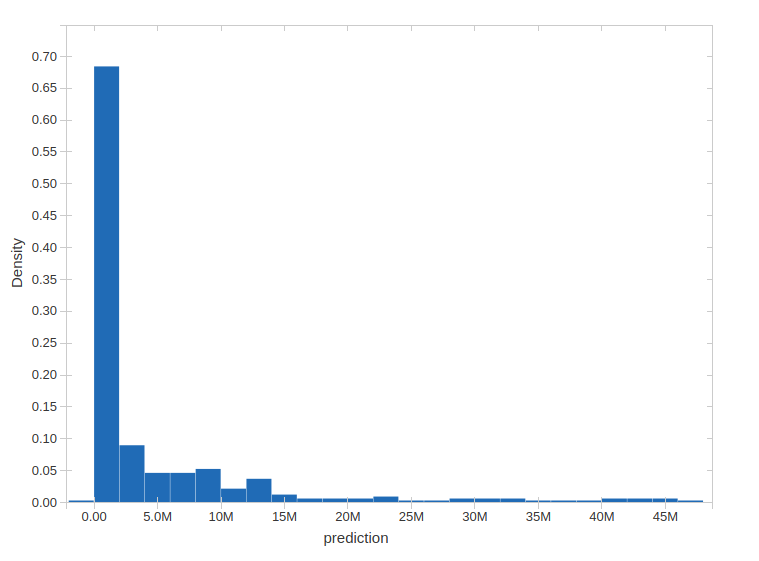
\includegraphics[width=0.5\textwidth]{predicted.png}
\end{figure}

\begin{figure}[h]
\caption{Actual Settlement Values}
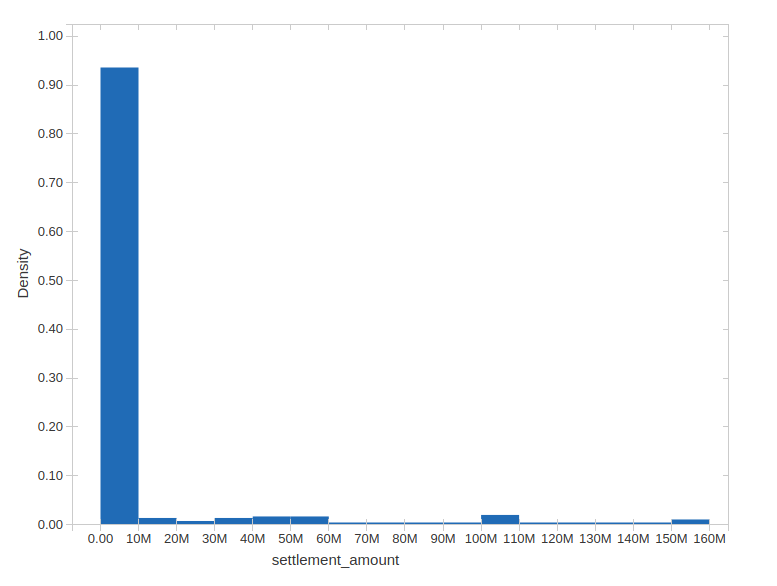
\includegraphics[width=0.5\textwidth]{actual.png}
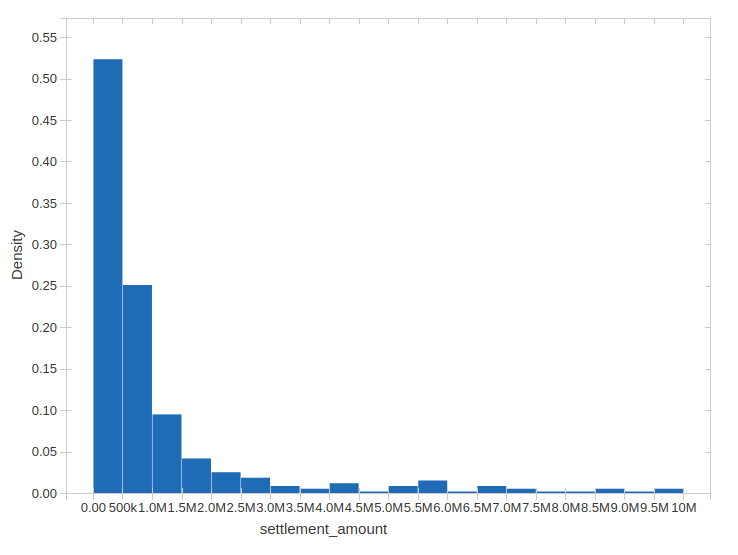
\includegraphics[width=0.5\textwidth]{actual2.png}
\end{figure}

The results, as mentioned, generally match the actual settlement values. However it would probably be worth continuing to tinker with the model and other regression models to determine whether we have the best fit here. We'd also like to note that for the purposes of this analysis settlements with multiple officers are effectively counted more than once, as each officer will show up in the data. To fix this in the future we could scale the settlements (i.e. a \$10 million settlement with two officers would be split into \$5 million settlements), but that has it's own problems. We could also just combine the stats of the officers into one row, but that again would introduce some issues, so for now at least we left it as is.

Looking at the error plot for the output test values, the model does well for smaller valued settlements but has problems with the larger settlements. This isn't unexpected, the larger values might be considered outliers and so don't fit in the model, but there are enough that I would be wary to exclude them.

\begin{figure}[h]
\centering
\caption{Error on predicted values}
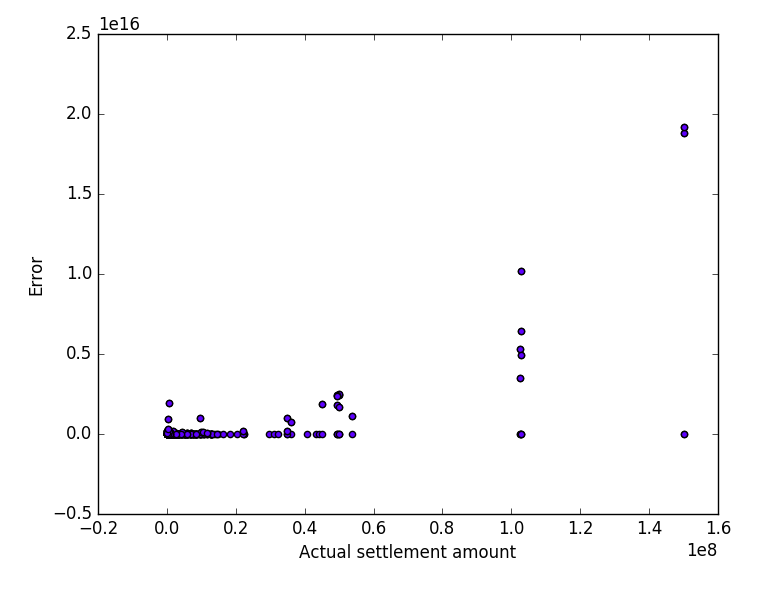
\includegraphics[width=0.5\textwidth]{errplot.png}
\end{figure}



\end{document}